% #############################################################################
%															Bahnplanung und Steuerung
% #############################################################################
\chapter{Bahnplanung und Steuerung}
\label{bahnplanung_steuerung_cha}

% ********************************************************************************
% 										Aufgabenstellung
% ********************************************************************************
\section{Aufgabenstellung}
\label{bahnplanung_aufgabenstellung_sec}
\authorsection{\editoroier}


Was die Aufgabestellung für betrifft, so soll der Roboter einen Menschen sicher und elegant, sprich ohne ruckartige Richtungswechseln, folgen können. Dabei soll es sicher durch die Innenräume fahren ohne mit Hindernissen zu kollidieren. Den abgefahrenen Pfad sollte dabei gespeichert werden, damit der Roboter später von alleine zur Startposition zurückkehren kann und danach vielleicht den gleichen Weg nochmal abfahren kann.


Für die Bahnsteuerung und Bahnplanung ist eine Einteilung in Abstraktionsschichten sinnvoll, da es der zu lösende Aufgabe hilft.
\begin{itemize}
	\item Motoransteuerung
	\item inverse Kinematik und manuelle Steuerung
	\item Bahnplanung	
\end{itemize}
Zusätzlich ist eine Simulation notwendig.

Für die Motoransteuerung ist die plattformspezifische Ansteuerung und Simulation notwendig. Außerdem sollte man auch die Pose aus Odometriedaten bestimmen können.

Die inverse Kinematik dient dazu, die erforderliche Gelenkeinstellung und Motorbewegungen zu berechnen, um zu einer bestimmten gewünschte Roboterpose zu gelangen. Probleme gibt es wenn es Raumpunkte gibt die zu Singularitäten führen. Das heißt, dass zum Beispiel bei einem 6-achsigen Roboter zwei Achsen kollinear werden. Die Vorwärtskinematik hingegen berechnet die Roboterpose auf Basis der interne Gelenkeinstellungen und Sensoren. Bei mobilen Robotern wird das auch Odometrie genannt.

Im Falle einer mobilen Plattform spricht man eher von Bahnplanung anstatt inverse Kinematik. Bei dieser Art von Robotern arbeitet die Regelung, um die geplante Bahn zu fahren, auf Basis der Odometrie in kartesische Koordinaten. Zu lösende Aufgaben im Bereich der inversen Kinematik sind: die Umrechnung der Trajektorie in Geschwindigkeiten, die Limitierung der Beschleunigung des Roboters und das Limitieren der Geschwindigkeiten unter Beachtung des Protective Fields \ref{sec:vpf}.

Was die Bahnplanung betrifft, gibt es mehrere Aufgaben. Als erstes müssen die Daten der Kinect-Kamera verarbeitet werden. 
Danach soll die Trajektorie, auf welcher der Roboter fahren soll, bestimmt werden, welches kollisionsfrei sein muss. Als letztes soll das 
Speichern der abgefahrenen Trajektorie und das Laden der abgefahrene Trajektorie implementiert werden.



% ********************************************************************************
% 										Grundlagen Bahnplanung
% ********************************************************************************
\section{Grundlagen der Bahnplanung und Steuerung}


\subsection{Steuerung}
\label{bahnplanung_steuerung_sec}

Weil die gefundene Trajektorie normalerweise nicht glatt ist, werden für die Steuerung unterschiedliche Interpolationsarten verwendet.
Die Bahnsteuerung kann im kartesischen Raum oder im Konfigurationsraum stattfinden.
Im kartesischen Raum ist es näher an der zu lösenden Aufgabe, man muss dann aber normalerweise für jeden Punkt die inverse Kinematik berechnen. Eine Ausnahme wären Radkinematiken bei mobilen Robotern. Bei mobilen Plattformen sind auch alle geplante Trajektorien ausführbar, insbesondere wenn sie omnidirektional sind, was bei Roboterarmen nicht der Fall ist. 
Die Steuerung im Konfigurationsraum hingegen liegt näher an den Gelenken, dafür ist die Formulierung der Trajektorie umständlicher.
Vor und Nachteile beider Optionen kann man in der Tabelle \ref{fig:steurungProContra} sehen.


\begin{table}[h]
		\centering
		\begin{tabular}{| p{7cm} | p{7cm}|}
\hline
\textbf{Kartesischer Raum} & \textbf{Konfigurationsraum}\\
\hline
+ Bahn einfacher zu formulieren & + Ansteuerung der Gelenke ist
einfacher\\
+ Interpolation ist einfacher & + Trajektorie ist eindeutig und
berücksichtigt Grenzen\\

- Inverse Kinematik ist für jeden Trajektorienpunkt zu lösen (außer bei mobilen Radkinematiken) & - Interpolation für mehrere
Gelenke\\
- Geplante Trajektorie nicht immer ausführbar (außer bei mobile Plattformen) & - Formulierung der Trajektorie umständlicher\\
\hline
		\end{tabular}
		\caption{\label{fig:steurungProContra} Vor und Nachteile der Steuerung im Kartesischen und Konfigurationsraum \citep{rob1}}
		\end{table}	
Es gibt unterschiedliche Interpolationsarten:
Zirkular, Linear und Spline-Bahn oder auch approximative Bahnsteuerung.
Bei der Linearinterpolation wird einfach zwischen zwei Teiltrajektorien interpoliert, wie man auf der Abbildung \ref{fig:linearinterpolation} sehen kann.
\begin{figure}[h]
	\center
	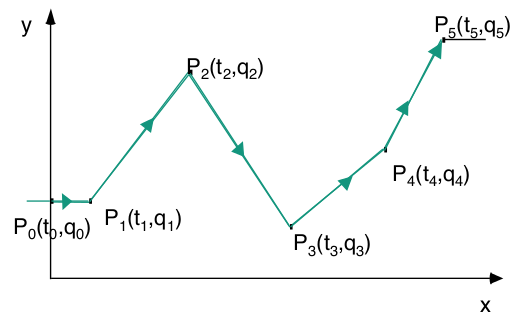
\includegraphics[scale=0.35]{graphics/linearinterpolation.png}
	\caption{\label{fig:linearinterpolation} Beispiel der Linearinterpolation Quelle: \citep{rob1}}
\end{figure}
Die Zirkularinterpolation schafft hingegen kreisförmige Verfahrwege zwischen zwei Punkten.
Wenn man allerdings segmentweise interpoliert, werden die Endbedingungen der Teiltrajektorie $i-1$ und die Anfangsbedingungen der Teiltrajektorie $i$ aneinander angepasst, so dass die Teiltrajektorien durch Splines beschrieben werden, wie man auf der Abbildung \ref{fig:segmentinterpolation} sehen kann.
\begin{figure}[h]
	\center
	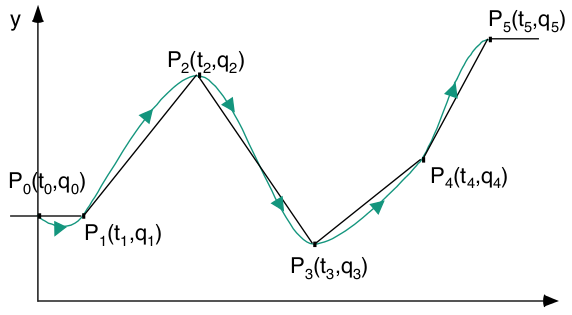
\includegraphics[scale=0.35]{graphics/segmentinterpolation.png}
	\caption{\label{fig:segmentinterpolation} Beispiel der segmentweisen Bahninterpolation \citep{rob1}}
\end{figure}
 
Bei der approximativen Bahnsteuerung werden anders als bei der Bahninterpolation nicht alle Kontrollpunkte der Trajektorie befahren, sondern die Kontrollpunkte beeinflussen den Bahnverlauf und werden approximiert.
Neben Bernsteinpolynomen wird hier besonders Überschleifen benutzt, um sanft Kurven zu fahren wie man auf der Abbildung \ref{fig:ueberschleifeninterpolation} sieht.
Letzteres wurde auch im Praktikum eingesetzt.
\begin{figure}[h]
	\center
	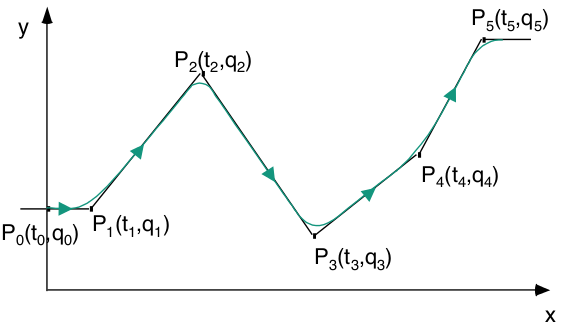
\includegraphics[scale=0.35]{graphics/ueberschleifeninterpolation.png}
	\caption{\label{fig:ueberschleifeninterpolation} Beispiel der approximierten Bahnsteuerung mit Überschleifen \citep{rob1}}
\end{figure}

\subsection{Bahnplanung}
\label{bahnplanung_grundlagen_sec}
\authorsection{\editoroier}

Bahnplanung befasst sich mit dem Problem, eine kollisionsfreie Bahn zu finden, die ein Robotersystem von der aktuellen Position in die Zielposition überführt.
Damit gehört es zu einer der Basisprobleme der Robotik.
Die Verfahren kann man nach unterschiedlichen Gesichtspunkten klassifizieren \cite{rob1}.

Nach Robotertyp:
\begin{itemize}
\item Bahnplanung für Manipulatoren (\zB Schweißen bei Industrierobotern)
\item Bahnplanung für mobile Roboter
\item Bahnplanung für Laufmaschinen und anthropomorphe Systeme
\item Greif- und Montageplanung
\end{itemize}

Nach dem Zustandsraum wo die Planung stattfindet:
\begin{itemize}
\item Gelenkwinkelzustandsraum (Konfigurationsraum,\\ der alle möglichen
Gelenkwinkelkonfigurationen des Roboters beinhaltet)
\item Euklidischer Raum (Arbeitsraum, 3D / 6D)
\item Sensorzustandsraum
\item Objektzustandsraum
\end{itemize}

Nach Vollständigkeit:
\begin{itemize}
\item Vollständige Verfahren (liefern immer eine korrekte Lösung und können ermitteln, ob keine Lösung existiert)
\item Probabilistisch vollständige Verfahren (Falls eine Lösung existiert konvergiert die Wahrscheinlichkeit, dass eine Lösung gefunden wird, bei fortschreitender Zeit gegen 1. Existiert keine Lösung, kann dies nicht ermittelt werden)
\end{itemize}

Nach Navigationsart:
\begin{itemize}
\item Globale Pfadplanung bedeutet, eine Trajektorie zum Ziel zu planen, wenn dem Roboter eine Karte der Umgebung vorliegt und er sich dort lokalisieren kann.
\item Lokale Pfadplanung wird eingesetzt um Hindernisse zu umfahren und wird bei mobilen Robotern meist in Kombination mit einem globalen Planer benutzt. 
\end{itemize}

Weil die explizite Berechnung des kollisionsfreien Konfigurationsraums bei Robotern mit mehr als drei Freiheitsgraden sehr teuer ist, benutzt man oft den impliziten Konfigurationsraum.
\Dh, dass die Bahnplanung im Konfigurationsraum stattfindet, aber die Kollisionen und Abstände im Arbeitsraum berechnet und in den diskretisierten Konfigurationsraum transformiert werden \citep{innoKonz}.
So wird der Konfigurationsraum während der Suche exploriert.

Der Ablauf eines Planungsverfahren ist normalerweise zweigeteilt\cite{Russell2003}.
\begin{enumerate}
\item Eine Roadmap oder einen Graph aufbauen mittels \gls{Voronoi},
 \gls{Sichtgraphen}, \gls{Zellenzerlegung} oder zufällige Knoten je nach
 Sampling-Strategie (\zB für \gls{PRM} Verfahren\cite{Thrun2005}).
\item Im Graph einen Weg vom Startknoten zum Zielknoten finden mittels A*-Algorithmus oder anderer Suchalgorithmen.
\end{enumerate}

\subsubsection{Lokale Planer}
\label{bahnplanung_lokale_planer_sec}

In diesem Abschnitt werden einige gängige lokale Planer vorgestellt.

\paragraph{A*-Algorithmus} 

Der \textit{A*-Algorithmus}\citep{Russell2003} ist eine Erweiterung des \textit{Dijkstra Algorithmus} und gehört zu der Klasse der informierten Graphensuchalgorithmen.
Dies heißt, dass eine Schätzungsfunktion benutzt wird, um die Suche zu lenken.
Die Grundidee ist, immer den Knoten zu untersuchen, der wahrscheinlich am schnellsten ins Ziel führt.
Um den vielversprechendsten Knoten zu ermitteln, werden alle bekannten Knoten mit einer $f(x)$ Funktion bewertet und vom kleinsten $f$-Wert zum größten sortiert.
Der Knoten mit dem kleinsten $f$-Wert wird als nächstes untersucht. 

Um den vielversprechendsten Knoten zu ermitteln, wird die Formel
\begin{equation}
 f(x) = g(x) + h(x)
\end{equation}
benutzt.
Dabei sind $g(x)$ die Pfadkosten, um $x$ vom Startknoten zu erreichen.
$h(x)$ ist die Heuristik, sprich die Schätzung der Pfadkosten, das Ziel von $x$ aus zu erreichen.
Wichtig dabei ist, dass die Heuristik immer optimistisch sein muss, das heißt, dass die Schätzung kleiner oder gleich sein muss als die wirklichen Pfadkosten, weil sonst der Algorithmus nicht mehr optimal ist.
Als Heuristik wird oft die \gls{Euklidische-Distanz} oder die \gls{Manhattan-Distanz} benutzt.
In Abbildung \ref{fig:a*} ist eine erfolgreich beendete \textit{A*}-Suche mit Angaben zum Ablauf dargestellt.

\begin{figure}[h]
\center
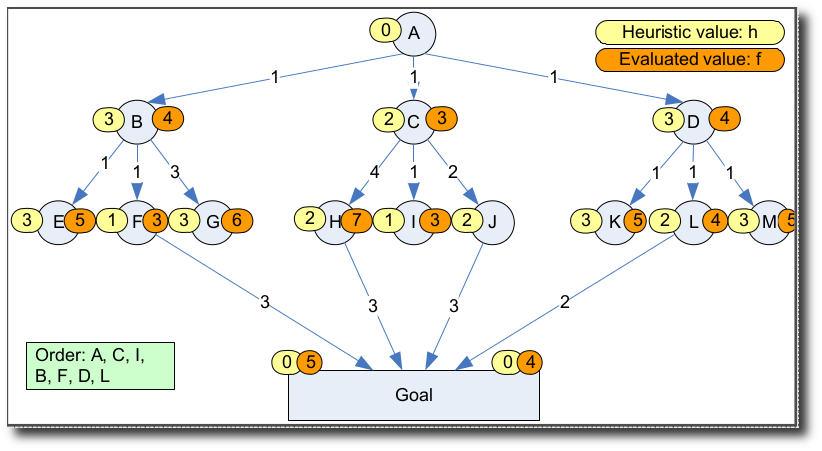
\includegraphics[scale=0.3]{graphics/AStar.png}
\caption{\label{fig:a*} Erfolgreich beendeter Ablauf eines \textit{A*}  \citep{innoKonz}}
\end{figure}

Der \textit{A*-Algorithmus}, obwohl er nicht mehr für bestimmte Anwendungszwecke als state-of-the-art gilt\citep{innoKonz}, ist als lokaler Planer, vor allem in 2D, sehr gut.
Mit mehr Dimensionen oder Freiheitsgraden arbeitet er viel schlechter. Als globaler Planer kann man es auch anwenden, zum Beispiel bei Navigationsgeräten. Diese benutzen Erweiterungen vom Grundalgorithmus, weil die Zustandsräume sehr komplex sind. 
Außerdem kann man den Grundalgorithmus noch weiter optimieren.
Zum Beispiel mit dem Hierarchischen \textit{A*}, damit er, wenn keine Hindernisse in der Nähe liegen, größere Schritte und sonst kleinere Schritte macht.
Es gibt zusätzliche Erweiterungen für die bidirektionale Suche, die parallele \textit{A*}-Suche und dynamische Auswahl von Start und Zielknoten.
Man könnte auch den Algorithmus stoppen, sobald man einen Weg gefunden hat, dann ist der Algorithmus natürlich nicht mehr optimal.
Diese Erweiterungen sind von der zu lösenden Aufgabe abhängig, mehrere Start und Zielknoten machen zum Beispiel bei mobilen Robotern nicht viel Sinn, dafür könnte es beim Schweißen nützlich sein.

\paragraph{Potentialfelder}

Bei diesen Verfahren bewegt sich der Roboter unter dem Einfluss von Kräften, die ein Potentialfeld auf ihn ausübt.
Die Grundidee ist, dass Hindernisse ein Abstoßungspotential auf den Roboter ausüben und das Ziel hingegen ein Anziehungspotential.
Der negative Gradient der resultierenden Potentialkraft bestimmt die künstliche Kraft, die auf den Roboter ausgeübt wird.

\begin{equation}
F(q) = - \nabla U(q)
\end{equation}
wobei $U(q)$ die Summe der Abstoßungs- und Anziehungspotentiale ist.
Diese Summe ist in Abbildung \ref{fig:potentialfeld} dargestellt.

\begin{figure}[h]
\center
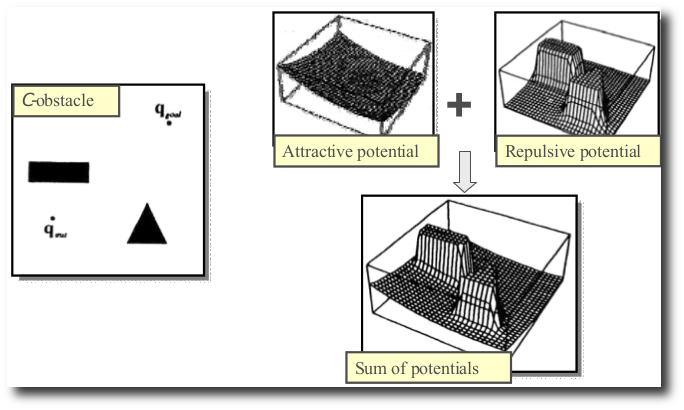
\includegraphics[scale=0.4]{graphics/potentialfeld.png}
\caption{\label{fig:potentialfeld} Summe der Abstoßungs- und Anziehungskräften \citep{innoKonz}}
\end{figure}

Die Vorteile des Verfahrens wären zum Beispiel der geringe Rechenaufwand für die Pfadplanung, dass die Bahnplanung und Steuerung in einer Funktion verbunden werden\citep{mobileRobotics}, was die allgemeine Steuerungsstruktur vereinfacht.
Noch ein Vorteil ist, dass die Pfade schon glatt sind, sprich man muss sie nicht mehr glätten.
Ein Nachteil hingegen ist, dass es im lokalen Minimum stecken bleiben kann.
Dies ist einer der Gründe, warum es als lokaler Planer benutzt wird.
Um dieses Problem zu beheben muss man Erweiterungen wie  \textit{random walk} oder \textit{backtracking} benutzen.
Eine andere Möglichkeit zur Flucht, die von Rimon und Koditschek vorgestellt wurde, ist es, den Zielpunkt als einziges lokales Minimum im Potentialfeld zu definieren.




% ********************************************************************************
% 										Umsetzung
% ********************************************************************************
\section{Umsetzung}
\label{bahnplanung_umsetzung_sec}


% -----------------------------------------------------------------------------
%													Motoransteuerung
\subsection{Motoransteuerung}
\label{bahnplanung_motoansteuerung_subsec}
\authorsection{\editoroier}



Was die Motoransteuerung angeht, so gab es schon das plattformunabhängige Modul
\lstinline{Segway-}\lstinline{OmniHal} von der Odete.
Unsere Aufgabe bestand darin, dieses Modul um die plattformspezifische Simulation \lstinline{Segway500RMPSimulation} zu ergänzen.
Als Eingaben erhält es Geschwindigkeiten, und Ausgaben sind die plattformspezifischen Geschwindigkeiten.
Auf der Abbildung \ref{fig:mca2architecture} sieht man die gesamte Struktur der Software und auf \ref{fig:segwayHal} ist das Modul \lstinline{SegwayOmniHal} abgebildet.

\begin{figure}[h]
	\center
	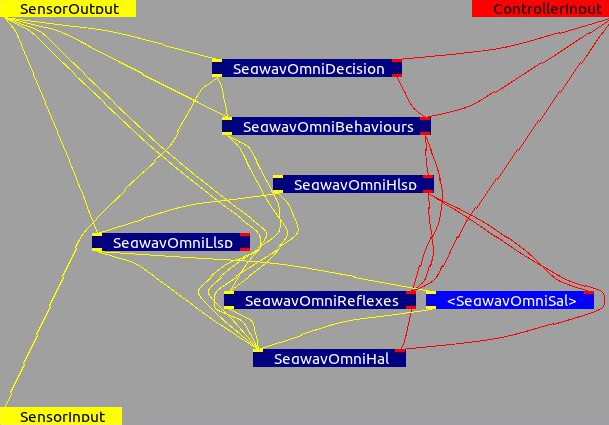
\includegraphics[scale=0.5]{graphics/mca2architecture.png}
	\caption{\label{fig:mca2architecture} Darstellung der Softwarearchitektur durch die vernetzten Gruppen.}
\end{figure}

\begin{figure}[h]
	\center
	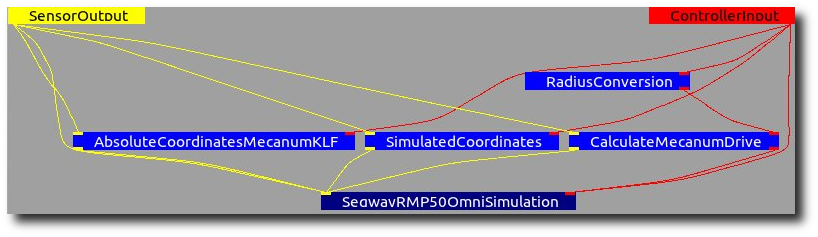
\includegraphics[scale=0.5]{graphics/segwayHal.png}
	\caption{\label{fig:segwayHal} Das Modul \lstinline{SegwayOmniHal}, welches für die Motoransteuerung zuständig ist.}
\end{figure}
% evtl. auch so ein Diagramm wie Abb. 4.4 von WS10/11?
%		bzw. Abb. 2.3 von WS09/10


% -----------------------------------------------------------------------------
%													Inverse Kinematik
\subsection{Inverse Kinematik und manuelle Steuerung}
\label{inverse_kinematik_subsec}
\authorsection{\editorjulian}
%\todo[inline]{Julian: Schreiben}
In der Gruppe \lstinline{SegwayOmniReflexes} befinden sich die Gruppen für die inverse Kinematik und die manuelle Steuerung des Roboters.
 Die Ausgaben der beiden Gruppen sind durch einen Multiplexer verbunden, die Selektion erfolgt durch die Berücksichtigung des Status der manuellen Steuerung.
 Ist diese aktiviert erfolgt unabhängig vom Zustand des Roboters das unmittelbare umschalten auf die manuelle Steuerung und die Ausgabe der Gruppe
 \lstinline{SegwayOmniManualReflexes} wird verwendet. Ist der manuelle Betrieb
 nicht aktiv kommt die Ausgabe der Gruppe
 \lstinline{SegwayOmni-}\lstinline{AutoReflexes} zur Verwendung. So ist es
 möglich zu jedem Zeitpunkt den Roboter zu stoppen und ihn manuell zu steuern.

\begin{figure}[h]
	\label{fig:bahnplanung_reflexes_gruppe}
	\center
	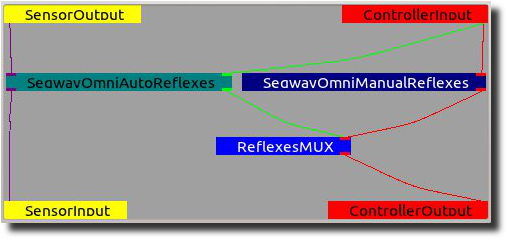
\includegraphics[scale=0.7]{graphics/BILD-SegwayOmniReflexes.png}
	\caption[Reflexes-Gruppe]{Die Gruppe \lstinline{SegwayOmniReflexes}, zu sehen sind die Gruppen für den manuellen bzw. automatischen Betrieb, \lstinline{SegwayOmniManualReflexes} und \lstinline{SegwayOmniAutoReflexes}.}
\end{figure}

Die manuelle Steuerung ist mittels der zur Simulation erstellten \lstinline{MCAGUI} Oberfläche oder - beim Test am realen Roboter - mit einem Gamepad möglich.

Die inverse Kinematik bezieht sich auf die \lstinline{MCA2}-Gruppe \lstinline{SegwayOmniAutoReflexes} in der die Umrechnung von einer Trajektorie, bestehend aus drei Koordinaten, in Geschwindigkeiten stattfindet. Die in dieser Gruppe berechneten Geschwindigkeiten sind plattformübergreifend; gehören allerdings einer bestimmten Bewegungsart an. Folgende Bewegungsarten sind bereitgestellt:

\begin{description}
	\item[Differentiell] Die Steuerung des Roboters erfolgt indem Antriebsräder auf beiden Seiten des Roboters mit unterschiedlichen Geschwindigkeiten betrieben werden\footnote{\url{http://en.wikipedia.org/wiki/Differential_wheeled_robot}}.
	\item[Omnidirektional] Durch den Einsatz von Mecanum-Rädern\footnote{\url{http://de.wikipedia.org/wiki/Mecanum-Rad}} kann sich der Roboter holonom\footnote{Anzahl der Bewegungsfreiheitsgrade $\geq$ Anzahl Freiheitsgrade, hier: Bewegungsfreiheitsgrade $= 3$, Freiheitsgrade $= 3$.} bewegen.
\end{description}

\begin{figure}[h]
\label{fig:bahnpl_umsetz_schema_inv_kinem}
\centering
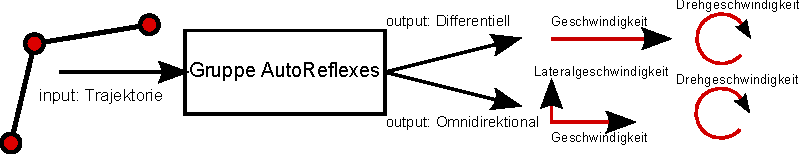
\includegraphics[width=\textwidth]{graphics/SCHEMA-invKinem.pdf}
\caption{Schematische Darstellung des in-und Outputs der \lstinline{SegwayOmniAutoReflexes}-Gruppe.}
\end{figure}

Zusätzlich zur Berechnung der Geschwindigkeiten erfolgt in dieser Gruppe die Begrenzung der tatsächlichen Geschwindigkeit bezüglich einer vorgegebenen maximal Geschwindigkeit sowie der auftretenden Beschleunigungen durch Änderungen der Geschwindigkeit oder Bewegungsrichtung.

Zuletzt findet mit Hilfe des Virtual Protective Field (siehe \ref{lokalisierung_umsetzung_sec}) eine Kollisionsvermeidung statt.

\begin{figure}[h]
	\label{fig:bahnplanung_umsetzung_auto_refl}
	\center
	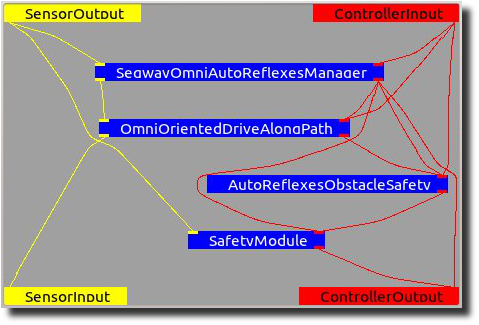
\includegraphics[scale=0.8]{graphics/BILD-SegwayOmniAutoReflexes.png}
	\caption[Reflexes-Gruppe im Detail]{Die Gruppe \lstinline{SegwayOmniAutoReflexes} im Detail. Auf oberster Ebene befindet sich das Manager-Modul, welches die einzelnen Module kontrolliert.}
\end{figure}

Die Ausgabe von dieser Gruppe, also die bewegungsartspezifischen Geschwindigkeiten, werden an die Gruppe für die Motoransteuerung (siehe \ref{bahnplanung_motoansteuerung_subsec}) weitergereicht, um plattformspezifische Geschwindigkeiten zu berechnen.

\subsubsection{Vorhandene Software}
\label{bahnplanung_inv_kinem_vorhandene_software_sec}

Im Projekt \lstinline{SegwayOmni} bzw. \lstinline{Odete} gab es bereits eine \lstinline{Reflexes}-Gruppe in der ein Großteil der nötigen Funktionalität implementiert war.
 Insbesondere der zentrale Teil, die Module
 \lstinline{DriveAlong-}\lstinline{Path} bzw.
 \lstinline{OmniOrientedDriveAlongPath} welche für die inverse Kinematik zuständig sind, wurden zur Verfügung gestellt. Auch die Module zur Begrenzung der Beschleunigung waren vorhanden verursachten im laufenden Betrieb allerdings Probleme.

\subsubsection{Erweiterungen}
\label{bahnplanung_inv_kinem_erweiterung_sec}

Um eine einfache Steuerung der Gruppe zu gewährleisten steht an oberster Stelle das Modul \lstinline{AutoReflexesManager}. Dieses Modul vereinfacht und automatisiert verschiedene Funktionen der Module \lstinline{DriveAlongPath}, \lstinline{OmniOrientedDriveAlongPath}, \lstinline{SafetyModule} und \lstinline{ObstacleSafety}:
\begin{description}
	\item[DriveAlongPath]
	\begin{itemize}
		\item Setzen der maximal Geschwindigkeit
		\item Aktualisieren des Zählers zum Signalisieren das eine neue Trajektorie anliegt
		\item Aktivieren/Deaktivieren des Moduls
	\end{itemize}
	\item[SafetyModule] 
	\begin{itemize}
		\item Aktivieren/Deaktivieren des Moduls
	\end{itemize}
	\item[ObstacleSafety] 
	\begin{itemize}
	\item Aktivieren/Deaktivieren des Moduls	
	\end{itemize}
\end{description}
Weiterhin fließt in der \lstinline{AutoReflexes}-Gruppe die Information aus dem Virtual Protective Field mit ein, um kollisionsfreies Fahren zu ermöglichen.

\subsubsection{Virtual Protective Field}
\label{bahnplanung_virtual_protective_field_sec}

Das Modul \lstinline{ObstacleSafety} ist speziell für den Einsatz beim omnidirektionalen Fahren gedacht. In diesem Fahrmodus berechnet sich der tatsächliche Geschwindigkeitsvektor aus zwei orthogonalen Geschwindigkeitsvektoren, die jeweils die Vorwärtsgeschwindigkeit und die Lateralgeschwindigkeit beschreiben. Das Virtual Protective Field bietet gleichermaßen, zu jeder Geschwindigkeitskomponente sowie zur resultierenden Geschwindigkeit, die Information ob eine Kollision bevorsteht. Dadurch kann für jede Geschwindigkeitskomponente individuell entschieden werden, ob es nötig ist diese auf null zu setzen, also mit maximaler Bremsbeschleunigung zu bremsen, oder nicht. Durch dieses Vorgehen kann sich der Roboter an Ecken, die durch ungenaue Bahnplanung zu einer Kollision führen würden, vorbei schieben. Zugleich ist es die letzte softwareseitige Barriere, um eine Kollision zu vermeiden. Dies tritt dann ein, wenn für jede Geschwindigkeitskomponente, sowie für den resultierenden Geschwindigkeitsvektor ein Hindernis gemeldet wird.

\begin{figure}
	\label{fig:bahnplanung_umsetzung_vpf}
	\centering
	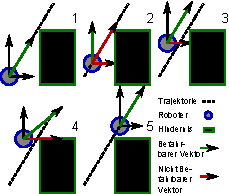
\includegraphics[scale=2]{graphics/SCHEMA-vpf.pdf}
	\caption[Einsatz des Virtual Protective Fields]{Schematische Darstellung wie das Virtual Protective Field eingesetzt wird um Kollisionen zu vermeiden.}
\end{figure}

% -----------------------------------------------------------------------------
%													Bahnplanung
\subsection{Bahnplanung}
\label{bahnplanung_subsec}
\authorsection{\editortobias}


% \begin{itemize}
% 	\item Kurzer Grobüberblick über die Behaviours-Gruppe, hier werden Bahnplanungs-Aufgaben bearbeitet\todoprivate{ref zu behaviours-Bild}
% 	\begin{itemize}
% 		\item Berechnung von Trajektorien-Punkten auf Basis der Mensch-Position und Geschwindigkeit (Kinect)
% 		\item Schätzung der zukünftigen Position des Menschen
% 		\item Transformation von Welt- in Roboter- bzw. Bildkoordinaten und zurück\todoprivate{evtl. auch weg lassen}
% 		\item Abspeichern von Pfaden
% 		\item Abfahren von Pfaden
% 	\end{itemize}
% 	\item Module werden im Folgenden kurz beschrieben
% 	\item Kollisionsvermeidung als eigener Abschnitt
% \end{itemize}

Die Aufgaben der Bahnplanung werden in der \lstinline{MCA2}-Gruppe \lstinline{SegwayOmniBehaviours} bearbeitet (s. Abb. \ref{fig:behaviours}).
Im Einzelnen sind dies:
\begin{itemize}
	\item Berechnung von Trajektorien-Punkten auf Basis der Mensch-Position und Geschwindigkeit: \lstinline{GenerateTrajectory}
	\item Schätzung der zukünftigen Position des Menschen: \lstinline{HumanPosition}
	\item Abspeichern von Pfaden: \lstinline{StoreRoboterPositionsToFile}
	\item Abfahren von Pfaden: \lstinline{LoadRoboterPositionsFromFile}
	\item Kollisionsvermeidung: \lstinline{ObstacleAvoidance}
\end{itemize}

\begin{figure}[h]
	\center
	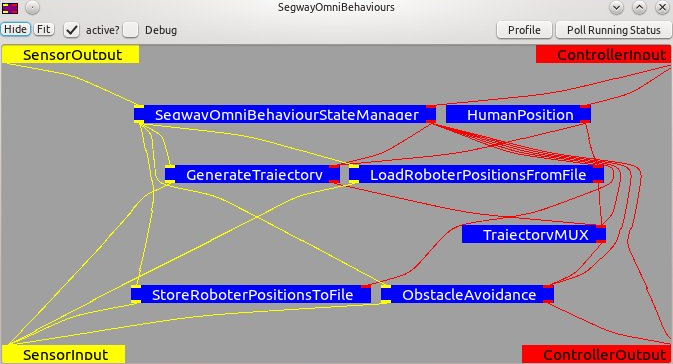
\includegraphics[width=0.8\textwidth]{graphics/behaviours}
	\caption{Die \lstinline{MCA2}-Gruppe \lstinline{SegwayOmniBehaviours}}
	\label{fig:behaviours}
\end{figure}

Die Module innerhalb der Gruppe werden im Folgenden beschrieben.
Die Kollisionsvermeidung wird in einem gesonderten Abschnitt (s. Abs. \ref{kollisionsvermeidung_subsec}) behandelt.


\subsubsection{Position des Menschen}
\label{bahnplanung_humanPosition_subsubsec}

% \begin{itemize}
%     \item bekommt aktuelle Position und Geschwindigkeit des Menschen von Kinect
%     \item schätzt die zukünftige Position des Menschen anhand dieser Daten
%     \item gibt aktuelle und geschätzte Position des Menschen aus
%     \item Zeit-Parameter für die Schätzung: $t_{est}$
%     \item Berechnung nach der Formel: $s_{est} = s_{act} + v \cdot t_{est}$
% \end{itemize}

Das Modul \lstinline{HumanPosition} bekommt als Parameter die aktuelle Position sowie die aktuelle Geschwindigkeit der vom Roboter verfolgten Person übergeben.
Anhand dieser Daten wird die zukünftige Position des Menschen geschätzt.
Als Resultat gibt das Modul die geschätzte zukünftige Position des Menschen aus.
Die aktuelle Position wird ebenfalls mit ausgegeben.

Für die Berechnung der zukünftigen Position des Menschen wird die Formel
\begin{equation}
	s_{est} = s_{act} + v \cdot t_{est}
\end{equation}
angewendet.
$s_{est}$ ist dabei die geschätzte zukünftige Position, $s_{act}$ beschreibt die aktuelle Position und $v$ die Bewegungsgeschwindigkeit des Menschen.
$t_{est}$ ist ein Parameter für die Zeitspanne, die in die Zukunft prädiziert werden soll.
Dieser Parameter wird aus einer externen Konfigurationsdatei geladen.


\subsubsection{Berechnung der Trajektorie}
\label{bahnplanung_trajektorie_subsubsec}

Die Berechnung der Trajektorie erfolgt im Modul \lstinline{GenerateTrajectory}.
Die aktuelle und geschätzte Position des Menschen, sowie die aktuelle Position des Menschen werden als Parameter übergeben, und dienen als Grundlage für die Berechnung der Trajektorie.
Die Struktur der zu berechnenden Trajektorie $s$ ist durch das Modul \lstinline{OmniDriveAlongPath} (s. Abs. \ref{bahnplanung_motoansteuerung_subsec}) vorgegeben:

% \begin{equation}
% 	s =
% 	\begin{pmatrix} start \\ next \\ following \end{pmatrix} =
% 	\begin{pmatrix} x_{st} & y_{st} & 0 \\ x_{nx} & y_{nx} & yaw_{nx} \\ x_{fl} & y_{fl} & 0 \end{pmatrix}
% \end{equation}
% 
% \todo[inline]{welche Variante nehmen?}

\begin{equation}
	s =	\begin{pmatrix} start \\ next \\ following \end{pmatrix}
\end{equation}
mit 
\begin{equation}
	start = 		\begin{pmatrix}	x_{start} \\ y_{start}							\end{pmatrix},
	next = 			\begin{pmatrix} x_{next} \\ y_{next} \\ yaw_{next}	\end{pmatrix},
	following =	\begin{pmatrix}	x_{following} \\ y_{following}							\end{pmatrix}
\end{equation}

%\begin{wrapfigure}{r}{0.35\textwidth}
\begin{figure}[h]
	\center
	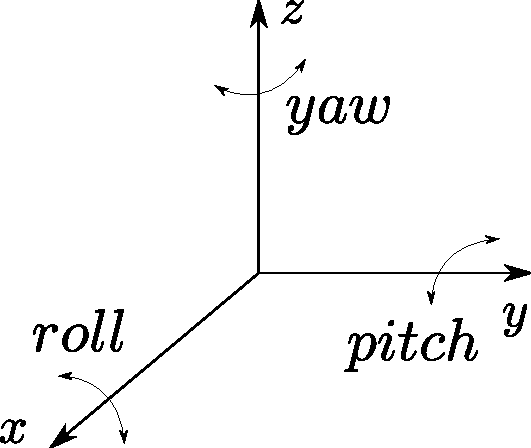
\includegraphics[width=0.3\textwidth]{graphics/roll_pitch_yaw.pdf}
	\caption{Roll-Pitch-Yaw-Winkel \cite{rollPitchYaw}}
	\label{fig:roll_pitch_yaw}
%\end{wrapfigure}
\end{figure}
Die drei Trajektorien-Punkte sind Ortsangaben mit einer $x$- bzw. $y$-Koordinate.
$following$ beinhaltet zusätzlich eine Komponente für $yaw$ (die ``Blickrichtung'' des Roboters, s. Abb. \ref{fig:roll_pitch_yaw}).
Die Berechnung einer neuen Trajektorie wird durchgeführt, sobald neue Daten von \lstinline{HumanPosition} vorliegen.
Als $start$-Punkt wird dabei die aktuelle Roboterposition verwendet.
$next$ ist eine Roboter-Pose, die sich im Abstand $d_{hum}$ vor dem Menschen auf dem Vektor Roboter-Mensch befindet.
Im Abstand $d_{hum}$ vor der geschätzten zukünftigen Mensch-Position auf dem Vektor next-estimated befindet sich der dritte Punkt der Trajektorie: $following$.
Der Abstand $d_{hum}$ zum Menschen kann dabei als externer Parameter vorgegeben werden, der Wert beträgt standardmäßig $1,75m$.
In Abb. \ref{fig:trajektorie} wird dies in einer Schemazeichnung dargestellt.

\begin{figure}
	\center
	% Trajektorien-Punkte der Bahnplanung
% Author : Tobias Roth

\newcommand\Punkt{\tikz[scale=0.07]\draw[thick](-1,-1)--(1,1)(-1,1)--(1,-1);} 

\begin{tikzpicture}


\def \dHum {1.5}

% Definition der Koordinaten für Roboter, Mensch_act und Mensch_est
\def \rX {0}
\def \rY {0}
\def \hActX {3}
\def \hActY {4}
\def \hEstX {8}
\def \hEstY {4}

% Setzen der Koordinaten für Roboter, Mensch_act und Mensch_est
\coordinate (r) at (\rX,\rY);
\coordinate (hact) at (\hActX,\hActY);
\coordinate (hest) at (\hEstX,\hEstY);

% Berechnung der Trajektorien-Punkte
\coordinate (trajPointA) at (r);
\coordinate (trajPointB) at (2.1, 2.8);	% hart codiert..
\coordinate (trajPointC) at (6.53095, 3.70137);	% hart codiert..

% Poitionen zeichnen
\node at (r) (R) {\Punkt};
\node[scale=0.9] at (r) [anchor=east] {$R$};
\node at (hact) (H_act) {\Punkt};
\node[scale=0.9] at (hact) [anchor=south east] {$H_{act}$};
\node at (hest) (H_est) {\Punkt};
\node[scale=0.9] at (hest) [anchor=south west] {$H_{est}$};

\node[scale=0.9] at (r) [anchor=west] {$A$};
\node at (trajPointB) (B) {\Punkt};
\node[scale=0.9] at (trajPointB) [anchor=north] {$B$};
\node at (trajPointC) (C) {\Punkt};
\node[scale=0.9] at (trajPointC) [anchor=north] {$C$};

% Vektoren zwischen Positionen
\path[name path global=rHact, -] (r) edge (hact);
\path[-] (hact) edge (hest);

% d_{Hum} zeichnen
\draw [name path global=hactCircle] (hact) circle (\dHum);
\draw [name path global=hestCircle] (hest) circle (\dHum);
\path[<->] (hact) edge node {$d_{hum}$} (\hActX,\hActY + \dHum);
\path[<->] (hest) edge node {$d_{hum}$} (\hEstX,\hEstY + \dHum);

% Eigentliche Trajektorie zeichnen
\path[red, thick, ->] (trajPointA) edge (trajPointB);
\path[red, thick, ->] (trajPointB) edge (trajPointC);



% Eigentliche Trajektorie zeichnen
% \path [name intersections={of=rHact and hactCircle, by={A}}];
% \node at (A) [below] {$A$};
% \path [name intersections={of=hactCircle and rHact}];
% \coordinate [label=above:$C$] (C) at (intersection-0);


\end{tikzpicture}

	\caption{Berechnung der Trajektorien-Punkte}
	\label{fig:trajektorie}
\end{figure}

Der $yaw$-Wert wird so berechnet, dass der Roboter sich immer in Richtung des Menschen ausrichtet.
So kann gewährleistet werden, dass die Kinect den Menschen weiterhin im Fokus hat.


% \begin{itemize}
% 	\item Modul bekommt aktuelle und geschätzte Position des Menschen, sowie aktuelle Position des Roboters
% 	\item Struktur der zu berechnenden Trajektorie duch \lstinline{OmniDriveAlongPath} \todoprivate{ref zu LowLevel?}\ vorgegeben:
% 	\begin{itemize}
% 		\item Start $(x,y)$, Koordinaten
% 		\item Following $(x,y,yaw)$, Koordinaten und Orientierung \todoprivate{Skizze zu x-y-z-roll-pitch-yaw ?}
% 		\item Next $(x,y)$, Koordinaten
% 	\end{itemize}
% 	\item Berechnung einer neuen Trajektorie, sobald neue Mensch-Daten vorliegen
% 	\item Berechnung der Trajektorien-Punkte im Einzelnen:
% 	\begin{itemize}
% 	  \item Start: aktuelle Roboterposition
% 	  \item Next: Pose auf Roboter-Mensch-Vektor, die sich im Abstand $d$ vor dem Mensch befindet; yaw wird gesondert berechnet, sodass Roboter immer zu Mensch schaut
% 	  \item Following: Position auf next-estimated-Vektor, die sich $d$ vor geschätzter Mensch-Position befindet
% 	  \item erfolgt alles in absoluten Weltkoordinaten
%   \end{itemize}
%   \item Parameter $d$ für den Abstand des Roboters zum Menschen, default: $1,75m$
%   \item Berechnung des yaw-Wertes: \todoprivate{Formel dazu}

% 	\item MUX für Trajektorie
% 	\begin{itemize}
% 		\item GenerateTrajectory
% 		\item LoadFromFile
% 	\end{itemize}
% \end{itemize}


\subsubsection{Pfadspeichern und -laden}
\label{bahnplanung_pfadSpeichernLaden_subsubsec}

% \begin{itemize}
%   \item Im \lstinline{followPerson} -Zustand: Wegpunkte $(x,y,yaw)$ werden in gewissen Abständen $d_{save}$ gespeichert
%   \begin{itemize}
%     \item sobald $ \overline{ s_{act} - s_{last} } > d_{save} $ \todoprivate{Fehler im Code??? Euklidischer Abstand stattdessen verwenden?}
%   \end{itemize}
% 	\item Im \lstinline{loadPath} -Zustand: Nächster Wegpunkt wird geladen, sobald vorheriger erreicht wurde
%   \begin{itemize}
% 		\item Im \lstinline{returnHome} -Zustand: Nächster Wegpunkt wird geladen, sobald vorheriger erreicht wurde; umgekehrte Reihenfolge
%     \item sobald $ d( s_{foll} - s_{act} ) < d( s_{nxt} - s_{act} ) $, Euklidischer Abstand
%   	\item \lstinline{yaw} wird unabhängig von Datei berechnet, sodass Roboter immer Menschen anschaut
%   \end{itemize}
%   \item Eigene Klasse zum File-Handling: \lstinline{fileUtil}
%   \begin{itemize}
%     \item Mehrere dump-files möglich
%     \item Auslesen der Wegpunkte in normaler und umgekehrter Reihenfolge
%   \end{itemize}
% \end{itemize}

Zur Pfadspeicherung bzw. zum Laden eines abgespeicherten Pfades werden zwei Module, sowie eine Helfer-Klasse verwendet:
\begin{itemize}
	\item \lstinline{StoreRoboterPositionsToFile}: Während dem Modus \lstinline{followPerson} (s. S. \pageref{integration_umsetzung_hierarchie_sec}, Abs. \ref{integration_umsetzung_hierarchie_sec} für weitere Informationen zur globalen Zustandsmaschine) aktiv
	\item \lstinline{LoadRoboterPositionsFromFile}: Während dem Modus Während dem Modus \lstinline{followPath} (s. Abs. \ref{integration_umsetzung_hierarchie_sec}) aktiv
	\item \lstinline{fileUtil}
\end{itemize}

Im globalen Modus \lstinline{followPerson} (s. Abs. \ref{integration_umsetzung_hierarchie_sec}), also während dem Einlernen eines neuen Pfades,
 schreibt das Modul \lstinline{StoreRoboterPositionsToFile} in regelmäßigen Abständen $d_{save}$ Roboterposen in eine externe Datei (sog. \lstinline{dumpFile}).
Für die Posen werden dabei sowohl die $x$- und $y$-Koordinaten, als auch die $yaw$-Werte abgespeichert.
Der Zeitpunkt für die Abspeicherung der nächsten Pose wird anhand der \glsdisp{Euklidische-Distanz}{Euklidischen-Distanz} festgelegt:
Sobald der Abstand der aktuellen Roboterpose zur letzten Speicherpose größer als der Speicherabstand $d_{save}$ ist, wird die aktuelle Pose abgespeichert.
$d_{save}$ kann als Parameter in einer externen Konfigurationsdatei definiert werden.
\begin{equation}
	\| s_{act} - s_{last}\|_2 \quad > \quad d_{save}
\end{equation}

Innerhalb des \lstinline{dumpFile}s werden die $x$, $y$ bzw. $yaw$-Werte zeilenweise durch Doppelpunkte getrennt gespeichert:
$x_i:y_i:yaw_i$

Im globalen Modus \lstinline{loadPath} (s. Abs. \ref{integration_umsetzung_hierarchie_sec}), also während dem Abfahren eines gespeicherten Pfades, liest das Modul \lstinline{LoadRoboterPositionsFromFile} die Punkte aus dem \lstinline{dumpFile}.
Die \gls{Euklidische-Distanz} findet wieder Verwendung, um den Zeitpunkt festzulegen, an welchem der nächste Punkt in die Trajektorie aufgenommen wird.
Dies geschieht, sobald der Abstand des Roboters zu $following$ kleiner ist als der zu $next$:
\begin{equation}
	\| s_{foll} - s_{act} \|_2 \quad < \quad \| s_{next} - s_{act} \|_2
\end{equation}
Im Modus \lstinline{returnHome} werden die Punkte in umgekehrter Reihenfolge ausgegeben.

In der aktuellen Implementierung werden die aus dem \lstinline{dumpFile} gelesenen $yaw$-Werte \emph{nicht} für die Trajektorie verwendet.
Grund hierfür ist die Entscheidung, dass der Roboter (bzw. die darauf installierte Kinect) immer den Menschen im Fokus behalten soll, um evtl. kurzfristige Stop-Kommandos empfangen und umsetzen zu können.
Die $yaw$-Werte, die während des Pfad-Einlernens abgespeichert wurden, beziehen sich auf die Standpunkte des Menschen zum dortigen Zeitpunkt, und nicht auf die aktuell relevanten Mensch-Positionen. 
Aus diesem Grund werden die $yaw$-Werte innerhalb des \lstinline{LoadRoboterPositionsFromFile}-Moduls auf Basis der aktuellen Mensch-Position gesondert berechnet.

Für die Aufgaben des Datei-Handlings wurde eine eigene Klasse implementiert, die Operationen wie Datei anlegen, öffnen, schließen, in die Datei schreiben, aus der Datei lesen etc. kapselt.
Hier werden die Daten aus der Datei gepuffert, sodass beispielsweise im Fall des Pfad-Lesens nur ein einmaliger Dateizugriff auf Betriebssystem-Ebene erfolgt.
Es ist auch möglich, mehrere \lstinline{dumpFile}s anzulegen.


% 
% % -----------------------------------------------------------------------------
% %													Transformationen
% \subsection{Transformationen}
% \label{transformationen_subsec}
% 
% \authorsection{\editorjulian}
% \todo[inline]{Julian: Sollen wir (also du ;-) ) noch so einen Abschnitt machen?}



% -----------------------------------------------------------------------------
%													Kollisionsvermeidung
\subsection{Kollisionsvermeidung}
\label{kollisionsvermeidung_subsec}

\subsubsection{Modul}
\authorsection{\editortobias}

% \begin{itemize}
%   \item Kollisionsvermeidungsmodul (\lstinline{ObstacleAvoidance}) überprüft die geplante Trajektorie auf Hindernisse, und plant ggf. um Hindernisse
%   \item Ausgaben von \lstinline{GenerateTrajectory} und \lstinline{LoadFromFile} werden geMUXt
%   \begin{itemize}
%     \item je nach Modus (\lstinline{followPerson} bzw. \lstinline{returnHome} / \lstinline{followPath}) schaltet MUX andere Eingänge durch
%   	\item Die Ausgabe des MUX wird dann widerum komplett durch das Kollisionsvermeidungsmodul (\lstinline{ObstacleAvoidance}) geschleift
%     \item Dadurch wird jede Trajektorie auf Hindernisse überprüft, keine kommt \glqq daran vorbei\grqq
%   \end{itemize}
%   \item Innerhalb des Moduls wird jede Trajektorie auf Hindernisse überprüft
% 	\begin{itemize}
% 	  \item die (Bild-)Punkte zwischen start, next und following werden berechnet (Transformation der Welt- in Bildkoordinaten)
% 	  \item Überprüfung für jeden einzelnen Punkt, ob er innerhalb eines Hindernisses liegt
% 	  \item Verwendung der \lstinline{ObstacleMap} \todoprivate{ref zu Lokalisierung}
% 	\end{itemize}
%   \item Ohne Hindernis werden Trajektorien-Punkte nur durchgeschleift
%   \item Wenn Hindernis erkannt, dann wird eine neue Trajektorie ermittelt
%   \begin{itemize}
%     \item Verwendung des A*-Algorithmus
%     \item Ermittlung des Start- und Endpunktes für A*
%     \item ggf. gesonderte Behandlung für Endpunkt (\lstinline{choosePointAfterObstacle})
%     \item Aufruf A*
%     \item Transformation der nuen Trajektorie IK $\rightarrow$ WK
%   \end{itemize}
% \end{itemize}

Das Modul \lstinline{ObstacleAvoidance} überprüft die geplante Trajektorie auf Hindernisse, und plant ggf. um ein Hindernis herum, um Kolissionen zu vermeiden.
Jede von \lstinline{GenerateTrajectory} bzw. \lstinline{LoadRoboterPositionsFromFile} (s. Abs. \ref{bahnplanung_trajektorie_subsubsec}) ausgegebene Trajektorie wird innerhalb des Moduls \lstinline{ObstacleAvoidance} auf Hindernisse überprüft, bevor sie an tiefer liegende Schichten weiter gegeben wird.
Dies wird durch einen \gls{mux} erreicht, der je nach globalem Modus die entsprechenden Eingänge an das Modul \lstinline{ObstacleAvoidance} durchschaltet.
So wird sichergestellt, dass ungeprüfte Trajektorien nicht an die Motoransteuerung weiter gegeben werden.
In Abb. \ref{fig:behaviours} (S. \pageref{fig:behaviours}) ist das Modul innerhalb der \lstinline{Behaviours}-Gruppe sichtbar.

Für die Hindernis-Überprüfung innerhalb des Moduls werden die Trajektorienpunkte, die alle in \gls{wk} vorliegen, in \gls{bk} transformiert.
So werden $start$, $next$ und $following$ auf entsprechende Punkte der \lstinline{ObstacleMap} (s. Abs. \ref{hinderniskarte_subsec}, S: \pageref{hinderniskarte_subsec}) abgebildet.
In einem weiteren Schritt werden alle \glstext{bk}, die zwischen den drei Trajektorienpunkten liegen, berechnet und in eine Liste geschrieben.
Die Punkte dieser Liste werden anschließend anhand der \lstinline{ObstacleMap} auf Hindernisse überprüft.

Falls für keinen der Punkte ein Hindernis festgestellt werden konnte, wird die Trajektorie (in \gls{wk}) unverändert weiter gegeben.

Liegt jedoch mindestens einer der Punkte innerhalb eines Hindernisses, so wird eine neue Trajektorie ermittelt, die um das Hindernis plant.
Hierfür wird der A*-Algorithmus verwendet.
Dieser benötigt einen Start- und einen Endpunkt, welche nicht innerhalb eines Hindernisses und auch nicht außerhalb des Bildes (\lstinline{ObstacleMap}) liegen dürfen.
Die Implementierung dieses Algorithmus wird im nächsten Abschnitt beschrieben.

Schließlich wird die durch den A*-Algorithmus neu berechnete Trajektorie in \gls{wk} umgerechnet, und an die Gruppe \lstinline{SegwayOmniReflexes} weiter gegeben.

\subsubsection{Algorithmus}
\authorsection{\editorjulian}
%\todo[inline]{Julian: Schreiben}
Um einen kollisionsfreien Pfad zu erstellen kommt eine Bahnplanungsmethode zum Einsatz, die den A*-Algorithmus verwendet.
Um den zeitlichen Aufwand einer eigenen Implementierung zu vermeiden wurde auf eine bereits existierende und frei verfügbare Implementierung von Justin Heyes-Jones\cite{jonesAstar} zurückgegriffen.
Diese Implementierung kann einfach eingebunden und erweitert werden.
Zum Einbinden des Algorithmus sind drei wesentliche Änderungen bzw.
Erweiterungen notwendig:
\begin{description}
	\item[Hinderniskarte] Eine Schnittstelle zur Verwendung eines \lstinline{CByteImage} als Hinderniskarte.
	\item[Heuristik] Ersetzen der ursprünglichen Heuristik durch die \gls{Euklidische-Distanz}.
	\item[Kostenfeld] Erweiterung um ein Feld, welches die Kosten zum Befahren eines bestimmten Punktes der Karte beschreibt.
\end{description}

Um beliebige Datencontainer als Hinderniskarte verwenden zu können wurde eine Interface-Klasse geschaffen.
Bei der individuellen Implementierung muss eine Funktion erstellt werden, die für eine Koordinate auf der Hinderniskarte die Information liefert ob sich dort ein Hindernis befindet oder nicht bzw.
wie \glqq teuer\grqq\ eine Fahrt dorthin ist.
Eine entsprechende Umsetzung wurde sowohl für ein \lstinline{CByteImage} als auch für ein \lstinline{IplImage} vorgenommen.

In der ursprünglichen Implementierung des A*-Algorithmus kommt als Heuristik, für die Distanz zwischen zwei Punkten, die \gls{Manhattan-Distanz} zur Verwendung.
Da sich der Roboter omnidirektional bewegen kann, ist es sinnvoll stattdessen die \gls{Euklidische-Distanz} zu verwenden.
\begin{figure}[h]
	\centering
	\label{fig:bahnplanung_umsetzung_algorithm}
	\subfloat[Ursrpüngliche Hinderniskarte]
	{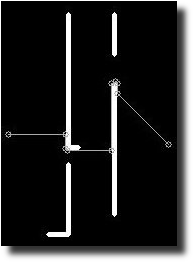
\includegraphics[scale=0.8]{graphics/BILD-Astar_normale_hindernisse.png}}
	\quad
	\subfloat[Hinderniskarte mit großen Hindernissen]
	{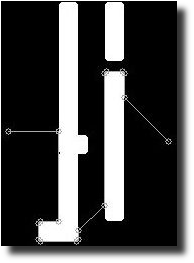
\includegraphics[scale=0.8]{graphics/BILD-Astar_grosse_hindernisse.png}}
	\quad
	\subfloat[Hinderniskarte mit Kostenfeld]
	{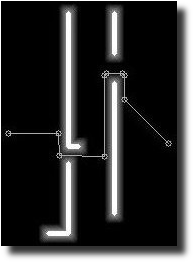
\includegraphics[scale=0.8]{graphics/BILD-Astar_antigrav.png}}
	\caption[Hinderniskarte und Trajektorie mit A*-Alg.]{Darstellung der Hinderniskarte und der gefundenen Trajektorie mit Hilfe des A*-Algorithmus, mit vergrößerten Hindernissen und mit Kostenfeld.}
\end{figure}
In der Praxis stellt sich bei der Verwendung des A*-Algorithmus heraus, dass die verwendete Implementierung zwar einen optimalen, also kürzesten Weg, findet, jedoch entspricht dieser Weg nicht immer der optimalen Näherung an eine direkte Verbindung.
Außerdem bewegt sich der gefundene Pfad häufig in direkter Nachbarschaft von Hindernissen.
Dieses Verhalten führte bereits in der Simulation zu erheblichen Problemen, kann allerdings durch die Erweiterung um ein Kostenfeld abgemildert werden.

Um einen gewissen Abstand zu den Hindernissen einzuhalten sind zwei Lösungen denkbar.
Die einfachste Variante ist es, die Hindernisse in der Hinderniskarte \glqq aufzublasen\grqq\ und so in der Realität für einen Mindestabstand zu sorgen.
Alternativ gibt es die Möglichkeit ein Kostenfeld einzusetzen. 

An engen Passagen auf der Hinderniskarte, bei denen der Roboter wenig Platz zu beiden Seiten hat, kommt es durch das Aufblasen der Hindernisse zu einem Verschluss dieser Passagen.
Das Finden eines Pfades ist dann unmöglich, da die ursprüngliche Passage nunmehr ein Hindernis ist.
Dies kann beispielsweise bei Türen der Fall sein.
Um diesem Problem zu begegnen kommt die zweite Lösungsmöglichkeit zur Verwendung.

Unter einem Feld versteht man in der Physik die räumliche Verteilung einer physikalischen Größe und speziell bei einem Skalarfeld die Zuordnung eines Skalars zu jedem Raumpunkt \cite{allgFeld},\cite{skalarFeld}.
Um das Finden eines Pfades zu verbessern, kann in einem solchen Feld zusätzliche Information über Hindernisse gespeichert werden.
Eine Möglichkeit zur Verwendung eines solchen Feldes, um sichere und weiche Trajektorien zu erstellen, kommt in \cite{Garrido2007} zur Sprache. In dieser Arbeit wird in einem ersten Schritt jedem freien Punkt der Hinderniskarte die Information abgelegt wie weit der nächste Hindernispunkt entfernt ist. Interpretiert in Form des Brechungsindex für elektromagnetische Wellen, kann in einem zweiten Schritt für jeden Punkt die Berechnung der Geschwindigkeit einer im Startpunkt ausgesendeten Wellenfront erfolgen. Die Trajektorie ergibt sich aus dem (zeitlich) kürzesten Weg um auf Basis dieser Ausbreitungsgeschwindigkeit vom Startpunkt zum Ziel zu kommen.

Im Rahmen des Praktikums wurde ein einfacherer Ansatz gewählt. Es kommt ein Kostenfeld zur Verwendung.
Der Begriff \glqq Kostenfeld \grqq\ bezieht sich auf die Tatsache, das der Wert den das Feld an einem bestimmten Punkt besitzt die Kosten repräsentiert die es benötigt auf auf diesen Punkt zu fahren.
In der Nähe von Hindernissen sind die Kosten hoch, in größerer Entfernung geringer.

Die Generierung des Kostenfeldes erfolgt, in dem jedem frei befahrbaren Punkt auf der Hinderniskarte, der sich noch in einem bestimmten Abstand zu einem Hindernispunkt befindet, ein Wert zugeordnet wird.
Dieser Wert verringert sich linear mit der Entfernung die dieser Punkt zum nächstgelegenen Hindernispunkt hat. So bietet jeder Punkt zusätzliche Informationen, die zur Pfadplanung verwendet werden können.
Konkret erfolgt die Realisierung durch das Belegen der Pixel mit Grauwerten, welche die Kosten repräsentieren die es benötigt um \glqq auf\grqq\ diesen Pixel zu fahren. Der Algorithmus versucht den günstigsten Weg zu finden und vermeidet das Fahren auf \glqq teuren\grqq\ Pixeln, die sich in der Nähe von Hindernissen befinden. Da es aber generell erlaubt ist auf diesen Pixeln zu fahren kann ein kollisionsfreier Pfad auch durch enge Passagen gefunden werden.



% -----------------------------------------------------------------------------
%													Simulation
\subsection{Simulation}
\label{simulation_subsec}
\authorsection{\editoroier}

Für die Simulation war schon eine Simulationsumgebung vorhanden.
Aufgabe war es, eine grafische Oberfläche mit Mcagui zu erstellen.
Die Simulation ist aus mehreren Gründen notwendig.
In erster Linie konnte man am Anfang am realen Roboter nicht testen, weil der Roboter noch gebaut wurde oder zum Beispiel nicht alle von uns programmierten Komponenten (wie bspw. die Lokalisierung) funktionsfähig waren.
Dank der Simulation wurde das Testen von einzelnen Funktionalitäten und die Darstellung des Roboterzustands möglich, wie man in Abbildung \ref{fig:mcagui} sehen kann.
\ZB wurde die Simulation sehr oft benutzt, um schnell Änderungen im Bahnplanungsalgorithmus zu testen.

\begin{figure}[h]
\centering
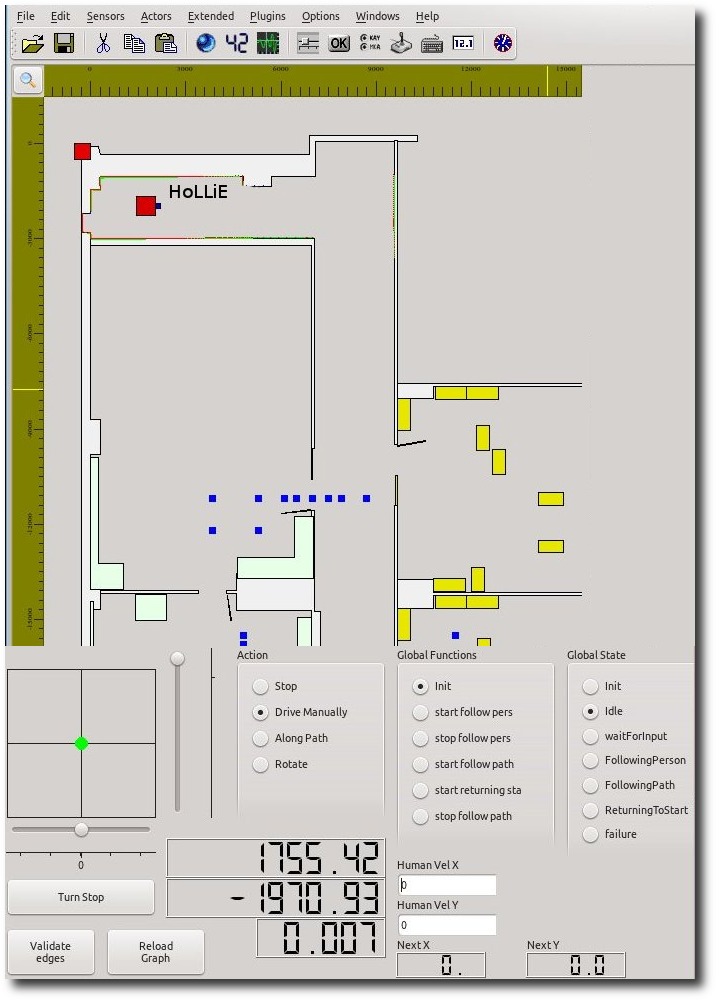
\includegraphics[scale=0.4]{graphics/mcagui_screenshot.png}		
\caption{\label{fig:mcagui} Die entwickelte Simulationsoberfläche
}
\end{figure}

Ein Problem am Anfang war, wie man den zu verfolgenden Menschen simulieren sollte.
Um dies zu lösen, benutzt man einfach Mausklicks auf der Karte.
